% Manuscript for Quantitative Science Studies. Build: paper/manuscript_qss/build.sh.
% Numbers come from paper/FINDINGS.md; figures from paper/figures (make_figures.py, make_tau_sweep.py).
\documentclass[11pt]{article}
\usepackage[margin=1in]{geometry}
\usepackage[T1]{fontenc}
\usepackage[utf8]{inputenc}
\usepackage{mathptmx}
\usepackage{microtype}
\usepackage{amsmath,amssymb}
\usepackage{graphicx}
\usepackage{booktabs}
\usepackage{threeparttable}
\usepackage[font=small,labelfont=bf]{caption}
\usepackage{setspace}
\usepackage[round,authoryear]{natbib}
\usepackage{xcolor}

\usepackage[hidelinks]{hyperref}

\usepackage{lineno}
\linenumbers
\onehalfspacing
\graphicspath{{../figures/}}

\newcommand{\PiP}{\mathrm{PiP}}
\newcommand{\Peers}{\mathcal{P}}

\title{Percentile in Percentile: rating scholars against their career cohort\\by the impact of their papers}
\author{Panos Ipeirotis\thanks{Department of Technology, Operations, and Statistics, Stern School of Business, New York University.}\textsuperscript{,}\thanks{Corresponding author: \texttt{panos@stern.nyu.edu}}
  \and Sen Tian\thanks{Ciphero.}}
\date{}

\begin{document}
\maketitle

\begin{abstract}
\noindent
Committees judge scholars early in their careers, before citations accumulate, but citation counts and the
$h$-index depend on field, grow with seniority and drift with the calendar. We propose PiP (percentile in percentile).
Each paper is ranked within its publication year. At every impact threshold above a cutoff, a scholar's count of
papers at or above it is ranked against peers who started in the same year; PiP averages these standings.
We compute PiP for 11.1 million Semantic Scholar authors. Paper percentiles at ages 3 and 10 correlate at 0.91,
and PiP's distribution barely changes across cohorts from 1960 to 2015, while the mean
$h$-index at career age 10 rose by about 40\%. PiP predicts a scholar's next ten years (number of top papers, chance
of an exceptional paper, citation impact) better than the $h$-index in every setting and in each of 15 fields. Under
the main eligibility rule, it finds future high performers as accurately as the $h$-index does at career age 10, but
1.6 to 1.8 years sooner. It better anticipates academy memberships, fellowships and prizes (AUC 0.75 against 0.71 at
career age 5), though only slightly within notable groups. The results hold without self-citations.
\end{abstract}

\noindent\textbf{Keywords:} research evaluation; citation percentiles; $h$-index; career age; indicators; Semantic
Scholar

\section{Introduction}

Hiring, promotion and award committees compare scholars with others at a similar career stage. A committee deciding on
tenure asks whether a candidate's record is strong for someone at that career stage; a funding panel compares
early-career applicants across departments. Bibliometric indicators enter these decisions alongside expert judgment. The
most common are citation counts and the $h$-index \citep{hirsch2005index}, whose values depend on the field, grow with
seniority and drift with the calendar. The average $h$-index ten years into a career is 40\% higher for scholars who
started in 2010 than for those who started in 1960 (Section~\ref{sec:cohorts}). A raw value says little until compared
with those of comparable scholars.

Many of these decisions are made early. Committees for hiring, tenure, fellowships and early-career grants judge
scholars in the first years of their careers, when most of their papers are recent and few have had time to collect many
citations. An indicator is most useful here if, at year five, it already separates the scholars who will do well later
from those who will not. Early detection was one of our motivations.

The $h$-index also reads only part of a record. It is the largest $h$ such that $h$ papers have at least $h$ citations
each, the corner where a scholar's sorted citation curve crosses the diagonal. Papers below the corner do not count,
nor do the citations of papers above it beyond $h$: a scholar with one landmark paper and another with one average
paper both have $h = 1$. A recent paper counts only after collecting $h$ citations, however well it compares with
papers of its own age.

For single papers, percentiles make that comparison. A paper's percentile is the share of papers from its publication
year (and possibly its field) that it out-cites, so a one-year-old paper competes only with other one-year-old papers.
Percentiles have become an established normalization, which the Leiden Manifesto calls the most robust
\citep{bornmann2013use,waltman2016review,hicks2015bibliometrics}. They are less influenced than means by the skewed
tail of the citation distribution \citep{bornmann2013use}, need no assumption about how citations grow with age, and
do not change meaning with the calendar.

Combining paper percentiles into a scholar-level indicator is less settled. Sums such as I3
\citep{leydesdorff2011integrated} grow without bound with the number of papers, so many weak papers can outweigh one
strong paper. Means ignore volume altogether. Counts of papers in the top 10\%
\citep{waltman2012leiden,bornmann2014individual} use one threshold and discard everything below it.

We propose PiP, short for \emph{percentile in percentile}, which places a scholar's papers in percentiles of their
publication year and then the scholar in percentiles of their career cohort: the peers whose first paper appeared in
the same year. For each impact threshold $\theta$, we count the scholar's papers at or above percentile $\theta$; the
share of peers with fewer such papers is the scholar's standing at the threshold. Across all thresholds, the standings
form a curve (Figure~\ref{fig:curves}). PiP is the average height of this curve over the thresholds above a cutoff
$\tau$. Where the $h$-index reads one corner of a record, PiP reads the whole curve above the cutoff.

With $\tau = 0.5$, used throughout, only papers in the top half of their year can earn credit, and recent papers can
earn it as soon as they stand out among papers of their own age. A single paper in the top 1\% counts at every threshold
up to the 99th percentile, where most peers have nothing. Lowering $\tau$ moves weight towards the number of papers;
raising it, towards their impact. The cutoff is a dial between quantity and impact.

We compute PiP from the Semantic Scholar Academic Graph \citep{kinney2023semantic} for 11.1 million authors at career
ages 1 to 30 (years since their first paper). Authors with at least three articles and an $h$-index of at least three
are \emph{eligible} and enter the comparison. In each evaluation year, we reconstruct peers and percentiles from the
publications and citations up to that year. We make six contributions:
\begin{enumerate}
  \item \textbf{Definition and properties.} PiP is bounded, never decreases when a paper is added or its percentile
  rises (peers and other papers' percentiles held fixed), gives nothing to papers strictly below the cutoff, and reads
  as the probability that the scholar has more papers above a random impact threshold than a random peer
  (Section~\ref{sec:pip}).
  \item \textbf{Measurement over time.} Paper percentiles settle within three to five years, and the time they need
  differs by field (Section~\ref{sec:paperstability}); PiP's distribution changes little across career cohorts from
  1960 to 2015 (Section~\ref{sec:cohorts}); and a scholar's PiP is less stable over a career than their article
  count, more stable than their $h$-index, and more stable than their citations over horizons of ten years or more
  (Section~\ref{sec:careerstability}).
  \item \textbf{Prediction.} PiP predicts future top papers better than the $h$-index in every setting and field we
  test, whether the $h$-index is raw or a cohort percentile; under an eligibility rule that ignores citations, the lead
  at the same career age narrows but remains. Top-paper counts, percentile sums and percentile means each beat PiP on
  at most one of three outcomes (the number of top papers, their citation impact and the chance of an exceptional
  paper); PiP balances all three. Comparing the scholar with peers at every threshold, rather than once for the whole
  record, better predicts citation impact and exceptional papers in every cohort; comparing once does about as well on
  the number of top papers and in early detection (Sections~\ref{sec:prediction} and~\ref{sec:early}).
  \item \textbf{Early detection.} At the same career age and under the main eligibility rule, PiP identifies future
  high performers at least as accurately as the other indicators we test. It reaches the accuracy that the $h$-index
  has at career age 10, but 1.6 to 1.8 years sooner (Section~\ref{sec:early}).
  \item \textbf{Later recognition.} Measured early in a career, PiP anticipates later academy memberships,
  fellowships and prizes better than the $h$-index among all scholars, though only slightly within already notable
  groups. For this purpose the impact end of the dial works best (Section~\ref{sec:honors}).
  \item \textbf{Robustness.} The results hold without self-citations; PiP rankings from Semantic Scholar agree with
  those from author-curated Google Scholar profiles; and a field-normalized version removes most of the advantage of
  high-citation fields while largely preserving the order within a field
  (Sections~\ref{sec:fields}--\ref{sec:robustness}).
\end{enumerate}

An earlier version of this work \citep{tian2021predictability} studied the predictability of paper and scholar
percentiles on a smaller dataset of faculty at top US universities and rated scholars by summing their paper
percentiles. Its reviewers objected to the unbounded sum, the selected population and the lack of field-level results.
This paper replaces the sum with PiP, covers every author eligible in each evaluation year (including those who later
stop publishing) and reports results by field. An earlier, asymmetric form of the score was described by
\citet{ipeirotis2024pip} and is used by the website \url{https://www.pip-score.org} (formerly
\url{https://scholar.ipeirotis.org}); Section~\ref{sec:auc} explains why we replace it.
\section{Related work}
\label{sec:related}

\paragraph{The $h$-index and its variants.} The $h$-index \citep{hirsch2005index} combines the number of papers and
their citations into a single number and has been studied, criticized and modified at length. The $g$-index
\citep{egghe2006theory} credits the citations above the corner; the $m$-quotient \citep{hirsch2005index}, the
contemporary $h$-index \citep{sidiropoulos2007generalized} and $hI_{a}$ \citep{harzing2014hia} correct for career length
by dividing by career age or discounting old papers; \citet{kaur2013universality} rescale the $h$-index by the field
average. Most variants correlate highly with the original \citep{bornmann2011metaanalysis}. They keep its construction,
a count of papers above a scholar-specific citation threshold, and so its blindness to papers below the corner.
The $h$-index is also inconsistent: adding the same paper to two scholars can reverse their order
\citep{waltman2012inconsistency}. So is PiP (Section~\ref{sec:properties}).

\paragraph{Percentiles.} Percentile-based indicators compare each paper with a reference set of papers from the same
year and field \citep{bornmann2013use,leydesdorff2011turning,waltman2013percentile,bornmann2020evaluation}. They are
less sensitive to outliers \citep{bornmann2013use,bornmann2020evaluation} than mean normalization, which compares a
paper's citations with the average of comparable papers \citep{schubert1986relative,Radicchi2008}. The Leiden
Manifesto recommends them \citep{hicks2015bibliometrics}. Ties and the definition of the percentile need care
\citep{waltman2013percentile}. For scoring we use the share of the reference set with strictly fewer citations, so that
uncited papers have percentile zero; for correlations, Hazen's mid-rank \citep{hazen1914storage}
(Section~\ref{sec:properties}).

\paragraph{From papers to scholars.} \citet{bornmann2014individual} propose counting a scholar's papers in the top 10\%
and dividing by career age, and I3 \citep{leydesdorff2011integrated,rousseau2012basic} sums percentiles over a set of
papers. Composite indicators such as that of \citet{ioannidis2019standardized} combine several citation counts, and
\citet{abramo2014productivity} relate field-normalized citations to the cost of labor. For countries and institutions,
double rank analysis expresses each paper's rank within its unit as a function of its rank among all papers in the
world; a power law fitted to this relation estimates the unit's chance of producing a very highly cited paper
\citep{rodriguez2018double,brito2018percentile}. PiP differs from these in normalizing twice: papers by publication
year, and the scholar by career cohort. The cohort comparison covers every impact threshold: the count of a scholar's
papers above each percentile is ranked among career peers, not read against the world distribution of papers.

\paragraph{Prediction of scholarly impact.} \citet{hirsch2007does} found that the $h$-index predicts a scholar's
later $h$-index and citations better than paper or citation counts do. Later work modeled impact as a stable individual
parameter applied to papers of random quality \citep{sinatra2016quantifying}, and \citet{clauset2017datadriven} review
the area. Other work predicted future $h$-index values from career features \citep{acuna2012future} and questioned how
much of that predictability is mechanical, because the future $h$-index contains the current one
\citep{penner2013predictability}. We avoid this overlap by predicting outcomes built only from papers published after
the evaluation year.

\paragraph{Citation windows and cumulative advantage.} How long a paper needs before its citations reflect its impact
depends on the field \citep{wang2013window,abramo2011window}. This matters for PiP, which scores recent papers by early
percentiles; Section~\ref{sec:paperstability} measures how fast they settle. Citations also feed on themselves:
well-known scholars receive more attention for the same work \citep{merton1968matthew,petersen2014reputation}. This
cumulative advantage affects any citation-based indicator and any test of its predictive validity
(Section~\ref{sec:discussion}).

\section{Data}
\label{sec:data}

\paragraph{Papers and citations.} We use the 27 October 2026 release of the Semantic Scholar Academic Graph
\citep{kinney2023semantic}, distributed under the ODC-BY license \citep{s2datasets2026}. It contains 226.0 million
papers published from 1950 to 2025. Counting each paper's citations by the year of the citing paper gives its
cumulative citations at each age $t$ (years after publication) through 2025. These counts sum to 97.5\% of the
citation counts that Semantic Scholar reports for papers from 2000--2005 (correlation 0.999); the difference consists
of citations from 2026 and from citing papers without a year.

\paragraph{Articles.} Many Semantic Scholar records are not research articles. We keep the 71.5 million papers typed as
journal articles, conference papers, reviews, studies, clinical trials, meta-analyses or case reports, and not as
editorials, news or letters. Only these \emph{articles} enter the reference sets, the paper counts and the $h$-index.
Of the records published in 2000, 63\% are uncited at age 5, but only 30\% of that year's articles. Each article
carries zero or more of Semantic Scholar's 23 fields of study \citep{s2graphapi}. From here on, \emph{papers} means
articles unless stated otherwise.

\paragraph{Authors and careers.} Semantic Scholar assigns author identifiers through automatic disambiguation
\citep{kinney2023semantic}. Disambiguation can split one person across several records or merge different people. We
link authors to their articles (277.8 million links). An author's \emph{start year} $s_a$ is the year of their first
article, and their \emph{career age} at evaluation year $Y$ is $A = Y - s_a$; an author who started in 1995 has career
age 10 in 2005. We follow every author from career age 1 to 30, or to 2025, whichever comes first.

Every quantity at evaluation year $Y$ is computed from the articles published up to $Y$ and their citations up to $Y$.
This reconstruction is retrospective in one respect: author identities, publication types and fields come from the
2026 release, not from the records of the time.

\paragraph{Eligibility.} At each evaluation year an author is \emph{eligible} if they have at least three articles and
an $h$-index of at least three, both computed from citations received through $Y$. The second condition means that at
least three of their articles have at least three citations each, so it implies the first. Because both counts only
grow, an eligible author remains eligible, even after they stop publishing. We compute PiP only for eligible authors
and compare each with their peers, the eligible authors who share their start year. In total, 11.1 million authors are
eligible at some career age, giving 111.6 million author-age records. The $h$-index condition is strict early in a
career and in slow-citing fields: among authors with start years 1975--2000 and at least three articles, it excludes
79\% at career age 3 and 43\% at career age 10, from 22\% in biology to 64\% in economics and 97\% in history and
philosophy. Sections~\ref{sec:early} and~\ref{sec:robustness} repeat the main comparisons under a
\emph{three-article rule}, which requires only the three articles.

\paragraph{Google Scholar profiles.} For validation we use 16,218 Google Scholar profiles, mostly of faculty, collected
for \url{https://www.pip-score.org}. Semantic Scholar's author records are built automatically, although authors can
claim and correct them \citep{kinney2023semantic}. Google Scholar profiles are created and curated by the scholars
themselves \citep{googlescholarprofiles}, so they are a check on automatic disambiguation
(Section~\ref{sec:robustness}). Section~\ref{sec:honors} also uses them in the test of later recognition.

\paragraph{Honors.} For the test of later recognition (Section~\ref{sec:honors}) we use Wikidata \citep{wikidata2026},
a free, collaborative knowledge base whose structured data are released under CC0. Items describing people can record
their honors, with dates, and their Semantic Scholar and Google Scholar identifiers. We queried Wikidata for honors on
5 November 2026. For the Google Scholar profiles we also record whether the scholar's item links to an English
Wikipedia article, using the website's monthly copy of Wikidata.
\section{The PiP score}
\label{sec:pip}

PiP makes two comparisons. It first ranks each of a scholar's papers against papers from the same year. It then counts
the scholar's papers at or above each impact threshold and ranks that count among peers, the scholars who started
publishing in the same year. The score averages these standings over the thresholds above a cutoff. We build it in
steps: the paper percentiles; the earlier form of the score, PiP-AUC, and why it rewards productivity more than impact;
and PiP, which removes that imbalance by comparing the scholar with peers at every threshold.

\subsection{Paper percentiles}
A paper one year old competes only with other papers one year old. Fix an evaluation year $Y$. For an article $j$
published in year $p_j \le Y$, let $c_j(Y)$ be its citations through $Y$. Its \emph{percentile} is the share of
same-year articles with strictly fewer citations at $Y$:
\begin{equation}
y_j(Y) = \frac{\left|\{\,i : p_i = p_j,\ c_i(Y) < c_j(Y)\,\}\right|}{\left|\{\,i : p_i = p_j\,\}\right|} \in [0, 1).
\end{equation}
Uncited articles have $y_j = 0$. Because the comparison stays within a publication year at a common evaluation time,
$y_j$ needs no correction for paper age or for citation growth over the decades. The main analysis pools all fields;
Section~\ref{sec:fields} computes percentiles within fields.

\subsection{Peers and the earlier score, PiP-AUC}
\label{sec:auc}
At evaluation year $Y = s_a + A$, the \emph{peers} $\Peers$ of author $a$ are the authors eligible at $Y$ with the same
start year, the author included. For an impact threshold $\theta \in [0,1]$, let
\begin{equation}
n_a(\theta) = \left|\{\, j \in a : p_j \le Y,\ y_j(Y) \ge \theta \,\}\right|
\end{equation}
count the author's articles at or above percentile $\theta$; $n_a(0)$ counts all articles, and $n_a(0.9)$ those in the
top 10\% of their publication year. For the median author of Figure~\ref{fig:curves}, $n_a(0) = 7$, $n_a(0.9) = 2$
and $n_a(0.95) = 1$.

The website \url{https://www.pip-score.org} uses the earlier form of the score, PiP-AUC \citep{ipeirotis2024pip}.
PiP-AUC compares the author with peers only through their total article counts. Let $F(m) = |\{b \in \Peers : n_b(0) \le
m\}| / |\Peers|$ be the productivity percentile, the share of peers with at most $m$ articles. With articles sorted by
percentile, $y_{(1)} \ge y_{(2)} \ge \cdots$, PiP-AUC is the area under the step curve of $y_{(k)}$ against $F(k)$:
\begin{equation}
\text{PiP-AUC}(a) = \sum_{k=1}^{n_a(0)} y_{(k)}\,\bigl[F(k) - F(k-1)\bigr] = \int_0^1 F\!\left(n_a(\theta)\right)
d\theta .
\label{eq:auc}
\end{equation}
It is the product of $F(n_a(0))$ and a weighted mean of the author's own percentiles, which keeps it bounded and
monotone. The second expression shows its asymmetry: at each threshold $\theta$, PiP-AUC compares the author's count at
or above $\theta$ with peers' \emph{total} counts rather than with their counts at or above $\theta$.

This asymmetry causes two problems. First, the score rewards productivity more than impact. The weight of the $k$-th
best article, $F(k) - F(k-1)$, is the share of peers with exactly $k$ articles, which is zero for every $k$ below the
smallest article count among peers. Among the eligible authors of a cohort, nobody has fewer than three articles, so an
author's best two articles receive no weight at all; among Google Scholar faculty profiles, the median author's best
four articles receive none. The productivity percentile accounts for 0.59--0.77 of the variance of the logarithm of
PiP-AUC. Scored against a simulated cohort of 2,000 peers, all with at least three articles, an author with one article
at the 99th percentile scores zero, while an author with 40 articles at the 10th percentile scores 0.10. Second,
applying a cutoff $\tau$ to this form makes it unstable across cohorts: it then compares partial counts with growing
total counts, and its median at career age 10 halves between the 1960 and 2010 cohorts. PiP removes both problems by
comparing like with like: at every threshold, the author's count at or above $\theta$ against peers' counts at or above
$\theta$.

\subsection{Standing curves}
The author's \emph{standing} at threshold $\theta$ is the share of peers with strictly fewer articles at or above
$\theta$:
\begin{equation}
g_a(\theta) = G_\theta\!\left(n_a(\theta)\right), \qquad
G_\theta(m) = \frac{\left|\{\, b \in \Peers : n_b(\theta) < m \,\}\right|}{|\Peers|}.
\end{equation}
For the median author, 63\% of peers have fewer than two articles in the top 10\%, so $g_a(0.9) = 0.63$. An author with
no article at or above $\theta$ stands at zero there, however many peers also have none (Section~\ref{sec:properties}).

Traced over all thresholds, the standings form the author's \emph{standing curve} $\theta \mapsto g_a(\theta)$. The
curve runs from the author's standing on the number of articles to their standing on the number of top articles, and
need not be monotone: an author can rank higher among peers on top-10\% articles than on all articles
(Figure~\ref{fig:curves}). The curve rises and falls in a sawtooth. Between two of the author's own article
percentiles, $n_a(\theta)$ stays constant as $\theta$ rises while peers' counts can only fall, so the standing can only
rise. It can fall only where $\theta$ passes one of the author's articles and $n_a(\theta)$ drops by one, and does so
unless peers' counts fall enough at the same threshold.

\begin{figure}[t]
  \centering
  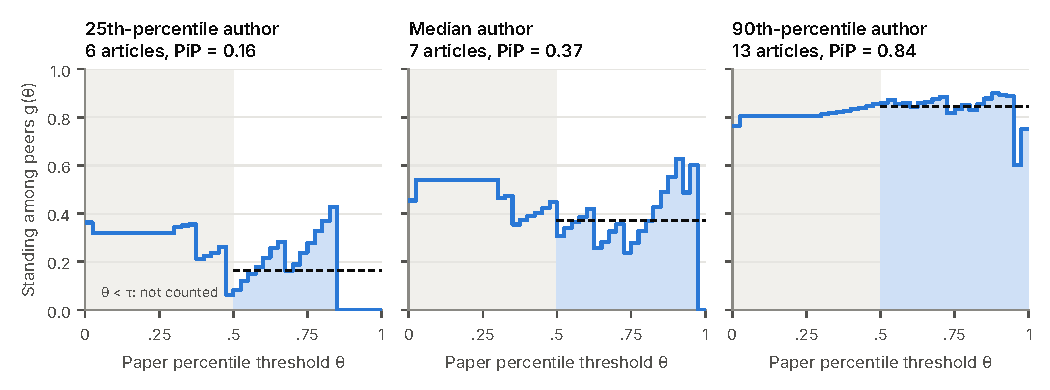
\includegraphics[width=\textwidth]{fig_standing_curves.pdf}
  \caption{Standing curves of three authors who published their first article in 1995, evaluated in 2005 (career age
  10). Each was chosen as the author whose PiP is closest to the 25th, 50th or 90th percentile of the cohort's scores.
  Each curve gives, at every threshold $\theta$, the share of the 1995 cohort's eligible authors who have fewer articles
  at or above percentile $\theta$ of their publication year. PiP is the shaded area to the right of $\tau = 0.5$,
  rescaled by $1/(1-\tau)$, or equivalently the average height of the curve there (dashed line). The ticks on the
  horizontal axis mark the author's articles; the curve can fall only at these ticks. The median author has seven
  articles, two of them in the top 10\% of their year and one in the top 5\%. At thresholds from 0.85 to 0.95 this
  author stands above 49\% to 63\% of the peers, who have fewer articles cited that highly.}
  \label{fig:curves}
\end{figure}

\subsection{Definition}
\label{sec:definition}
The PiP score with cutoff $\tau \in [0, 1)$ is the average standing over the thresholds at or above $\tau$:
\begin{equation}
\PiP_\tau(a) = \frac{1}{1-\tau} \int_\tau^1 g_a(\theta)\, d\theta .
\label{eq:pip}
\end{equation}
It is the area under the standing curve to the right of $\tau$, rescaled to $[0,1]$. The cutoff moves the score
between quantity and impact (Section~\ref{sec:tau}). We use $\tau = 1/2$ throughout and write PiP for $\PiP_{1/2}$.
With this cutoff, only articles in the top half of their publication year can earn credit.

The score is also the chance of winning a simple game. Draw a random peer and a random threshold from $[\tau, 1]$, the
range the cutoff sets. The author wins with strictly more articles at or above the threshold, so a tie is not a win.
Formally, if $B$ is a random peer and $\Theta$ a threshold drawn uniformly from $[\tau, 1]$, then
\begin{equation}
\PiP_\tau(a) = \Pr\left[\, n_a(\Theta) > n_B(\Theta) \,\right]:
\end{equation}
PiP is the probability that, above a random impact threshold, the author has more articles than a random peer.

The median author of Figure~\ref{fig:curves} wins against 63\% of peers when the threshold is at the 90th percentile
(the author has two articles there and most peers have fewer), against 28\% at the 75th percentile, and against none
at the 97.5th percentile. Averaged over thresholds above the cutoff, the author wins 37\% of the time, even though
their score is near the cohort median. A score of 0.6 therefore means winning 60\% of these matchups, not being at the
60th percentile of scores. At career age 10, across cohorts from 1960 to 2015, the lower quartile of PiP lies between
0.16 and 0.20, the median between 0.37 and 0.41, the upper quartile between 0.64 and 0.68 and the 90th percentile
between 0.84 and 0.86 (Section~\ref{sec:cohorts}), so a score of 0.6 lies between the median and the upper quartile of
its cohort.

Not counting ties as wins also determines a peer group's mean score. Let $p_{\theta,m}$ be the share of peers with
exactly $m$ articles at or above $\theta$. Two random peers tie at $\theta$ with probability $\sum_m p_{\theta,m}^2$
and are otherwise equally likely to lead, so averaging over peers gives
\begin{equation}
\frac{1}{|\Peers|} \sum_{a \in \Peers} \PiP_\tau(a)
= \frac{1}{2(1-\tau)} \int_\tau^1 \Bigl(1 - \sum_m p_{\theta,m}^2\Bigr)\, d\theta .
\label{eq:mean}
\end{equation}
This mean is below one half and falls as ties become more common, as at high cutoffs (Section~\ref{sec:tau}).

To measure what the comparison at every threshold adds, Sections~\ref{sec:prediction} and~\ref{sec:early} also report
\emph{PiP-simple}. It keeps the paper percentiles and the cutoff but compares the scholar with peers only once,
through the rank of the score in the cohort: it sums the counts above the cutoff instead of the standings,
\begin{equation}
\text{PiP-simple}_\tau(a) = \frac{1}{1-\tau} \int_\tau^1 n_a(\theta)\, d\theta
= \frac{1}{1-\tau} \sum_j \max\left(y_j - \tau, 0\right).
\end{equation}

\subsection{Properties}
\label{sec:properties}
The properties below hold for a fixed peer group that contains the author; each follows in a line from the definitions.
We also checked them numerically on simulated cohorts (code in the replication package).

\paragraph{Range.} $0 \le \PiP_\tau(a) < 1$. The author is one of their own peers and never has fewer articles than
themselves, so $g_a(\theta) \le 1 - 1/|\Peers|$ at every threshold. The score is zero when, at almost every threshold
above $\tau$, no peer has a lower count than $a$, for example when every article of $a$ falls strictly below $\tau$.

\begin{table}[t]
  \centering
  \small
  \caption{Indicators as summaries of the count curve $n_a(\theta)$, the number of the author's articles at or above
  percentile $\theta$, and of the standing curve $g_a(\theta) = G_\theta(n_a(\theta))$.}
  \label{tab:taxonomy}
  \begin{tabular}{llll}
    \toprule
    Indicator & In terms of the curves & Thresholds used & Comparison with peers \\
    \midrule
    Article count & $n_a(0)$ & one ($\theta = 0$) & none, or once by rank \\
    Top-10\% count & $n_a(0.9)$ & one ($\theta = 0.9$) & none, or once by rank \\
    I3 & $\int_0^1 n_a(\theta)\,d\theta = \sum_j y_j$ & all & none, or once by rank \\
    PiP-simple$_\tau$ & $\frac{1}{1-\tau}\int_\tau^1 n_a(\theta)\,d\theta$ & $\theta \ge \tau$ & once, by rank \\
    $\PiP_\tau$ & $\frac{1}{1-\tau}\int_\tau^1 g_a(\theta)\,d\theta$ & $\theta \ge \tau$ & at every threshold \\
    \bottomrule
  \end{tabular}
\end{table}

\paragraph{Monotonicity.} With the peers and the percentiles of the author's other articles held fixed, adding an
article or raising an existing article's percentile never lowers $\PiP_\tau$: at every threshold either change raises
$n_a(\theta)$ or leaves it unchanged, and $G_\theta$ is non-decreasing. The gain can be zero: one more article at or
above $\theta$ raises the standing at $\theta$ only if some peer has exactly the author's previous count. An article
whose percentile stays strictly below $\tau$ changes $n_a(\theta)$ only for $\theta < \tau$ and leaves the score
unchanged. The property concerns percentiles, not raw citations: when a paper gains citations, its year's percentiles
are recomputed, and a paper that ties or overtakes another of the author's papers lowers that paper's percentile, so the
score can fall.

\paragraph{No reward for volume alone.} At $\tau = 1/2$, an author whose articles all fall below the median of their
year scores zero, however many they publish; under PiP-AUC, 40 articles at the 10th percentile score 0.10.

\paragraph{Credit for the best work.} A single highly cited article raises $n_a(\theta)$ by one at every threshold up
to its own percentile, including high thresholds where most peers have none. Scored against the simulated cohort of
Section~\ref{sec:auc}, which it does not join, a record of one article at the 97.5th, 99th or 99.9th percentile scores
0.42, 0.45 or 0.47, and one at the 50th percentile scores 0; PiP-AUC gives all four records zero. The
$h$-index cannot tell these records apart (all have $h = 1$).

\paragraph{Ties.} The standing counts peers with strictly fewer articles. Mid-ranks instead count half of the tied
peers. They are a common choice for the percentile of a single paper \citep{bornmann2013use,waltman2013percentile}, but
in the standing they would give credit to authors with nothing above a threshold: at high thresholds most peers have no
article, and an author tied with them at zero would stand at half their share. In the simulated cohort, an author whose
five articles all fall below the median would score 0.22 with mid-ranks instead of 0. The strict rule keeps weak
articles from earning credit through ties; its price is that the mean score of a peer group depends on how common ties
are (Eq.~\ref{eq:mean}).

\paragraph{Factorization.} PiP can be written as the author's productivity percentile $F$ (Section~\ref{sec:auc}) times
an impact multiplier. Unlike $G_\theta$, $F$ counts tied peers, so that it is positive for every member of the peer
group. Defining the \emph{impact multiplier} $Q_\tau(a) = \PiP_\tau(a) / F(n_a(0))$ gives
\begin{equation}
\PiP_\tau(a) = F\!\left(n_a(0)\right) \cdot Q_\tau(a).
\label{eq:factor}
\end{equation}
The identity holds by the definition of $Q_\tau$; it describes a score rather than explaining it. The multiplier
compares the author's standing on counts of articles above the cutoff with their standing on the number of articles,
and it exceeds one when the author ranks higher among peers on the former. Because $F$ counts ties and $G_\theta$ does
not, an author whose standing is the same at every threshold has $Q_\tau$ slightly below one.

In our data $Q_{1/2}$ exceeds one for 30--36\% of eligible authors, depending on career age. Across eligible authors
with a positive score who started in 1975--2005, at career ages 5, 10 and 20, the variance of $\log \PiP_{1/2}$ splits
into 0.74--0.82 from $\log Q$, about 0.30 from $\log F$ and a small negative covariance ($-0.04$ to $-0.11$). Most of
the variation in PiP across authors thus comes from the impact multiplier rather than from the number of articles. These
shares describe how scores vary, not how much of PiP reflects research quality.

\paragraph{Consistency.} PiP is not consistent in the sense of \citet{waltman2012inconsistency}: adding the same
article to two authors can reverse their order, because $G_\theta$ is not linear. In simulation, this happened in 0.7\%
of 3,000 random pairs. The $h$-index shares the property.

\subsection{Relation to other indicators}
\label{sec:relation}
Writing indicators in terms of the count curve $\theta \mapsto n_a(\theta)$ places PiP among existing ones. This curve
counts the author's articles at or above each threshold; PiP ranks this count among peers at every threshold above the
cutoff and averages the standings (Table~\ref{tab:taxonomy}). A top-$x\%$ count reads the curve at one threshold,
$n_a(1-x)$, without a peer comparison. I3 sums the percentiles, $\sum_j y_j = \int_0^1 n_a(\theta)\,d\theta$: the same
integral without the peer comparison, so it grows without bound with article count; PiP-simple applies this sum to the
articles above the cutoff, measured from the cutoff. The $h$-index reads one point of the analogous curve in citation
space, where the number of articles with at least $k$ citations equals $k$.

\section{Results}
\label{sec:results}

We first examine PiP as a measurement: how soon a paper's percentile settles, what the cutoff changes, whether a score
is equally rare in every cohort and how much it moves over a career. We then test whether PiP anticipates future work
and later honors, and check the findings by field and under other data choices.

\subsection{Paper percentiles settle within a few years}
\label{sec:paperstability}

PiP uses percentiles of recent papers, measured after only a few years of citations, so we check how well an early
percentile anticipates the later one. For every article published from 1980 to 1995, we compute its percentile within
its publication year at each age, correlate the percentiles at two ages within each year and average over publication
years. These percentiles are not the score's strict shares but Hazen mid-ranks \citep{hazen1914storage}, so the
correlation is the Spearman correlation of the citation counts.

\begin{figure}[t]
  \centering
  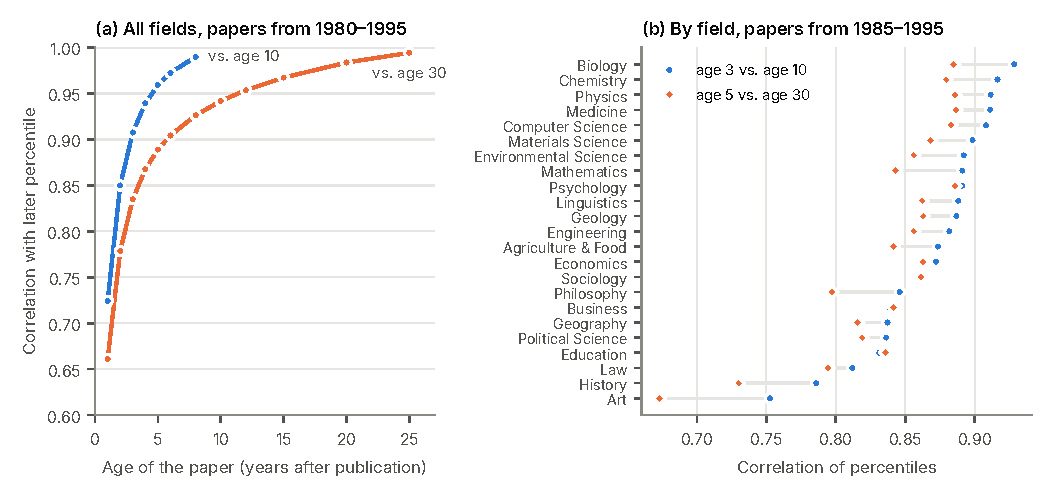
\includegraphics[width=\textwidth]{fig_paper_stability.pdf}
  \caption{How well a paper's early citation percentile anticipates its later percentile. (a) Correlation between
  the percentile at age $t_1$ and at age 10 or 30, for 7.2 million articles published in 1980--1995, averaged over
  publication years. (b) The same correlation by field, for articles published in 1985--1995, with percentiles
  computed within the field and publication year; fields with more than 20,000 articles.}
  \label{fig:paperstability}
\end{figure}

Percentiles settle quickly (Figure~\ref{fig:paperstability}a, Table~\ref{tab:paperstability}). The correlation with age
10 is 0.72 after one year, 0.91 after three and 0.96 after five; with age 30 it is 0.84 after three and 0.89 after five.
The ordinary least-squares slope of the later on the earlier percentile is close to one (0.94 for ages 3 and 10), so
early percentiles are not strongly biased towards the middle. Individual papers still move: between ages 3 and 10 a
paper's percentile changes by 0.086 on average (Table~\ref{tab:paperstability}).

The agreement between ages 3 and 10 holds in every publication year from 1960 to 1995: the correlation lies between
0.875 and 0.910. Early percentiles have also become more informative: the correlation between ages 1 and 10 was 0.72
for publication years 1980--1995 and 0.83 for 2015.

\begin{table}[t]
  \centering
  \small
  \caption{Agreement between a paper's citation percentile at an early and a later age (articles published 1980--1995,
  7.2 million articles). Correlation of Hazen percentiles within publication year, the slope of the later on the earlier
  percentile, and the mean absolute change.}
  \label{tab:paperstability}
  \begin{tabular}{lccc}
    \toprule
    Ages & Correlation & Slope & Mean absolute change \\
    \midrule
    1 vs.\ 10 & 0.724 & 0.846 & 0.161 \\
    2 vs.\ 10 & 0.850 & 0.911 & 0.115 \\
    3 vs.\ 10 & 0.908 & 0.944 & 0.086 \\
    5 vs.\ 10 & 0.959 & 0.975 & 0.051 \\
    3 vs.\ 30 & 0.835 & 0.882 & 0.125 \\
    5 vs.\ 30 & 0.889 & 0.918 & 0.100 \\
    10 vs.\ 30 & 0.942 & 0.956 & 0.068 \\
    20 vs.\ 30 & 0.984 & 0.989 & 0.030 \\
    \bottomrule
  \end{tabular}
\end{table}

The speed differs by field (Figure~\ref{fig:paperstability}b), in line with \citet{wang2013window} and
\citet{abramo2011window}. Three years give a correlation of about 0.9 with age 10 in biology (0.93), chemistry (0.92),
physics, medicine and computer science (0.91), but 0.79 in history and 0.75 in art. The humanities and law need about
five years to reach the agreement that the natural and life sciences reach in three. PiP uses each paper's percentile at
its current age, so in slow fields part of a scholar's score rests on unsettled percentiles;
Section~\ref{sec:discussion} discusses what this means for scholars in those fields.

\subsection{The cutoff $\tau$ is a dial between quantity and impact}
\label{sec:tau}

The cutoff decides which papers earn credit. To see how it moves the score between quantity and impact, we computed
PiP for $\tau \in \{0, 0.25, 0.5, 0.6, 0.75, 0.9\}$ for 3.43 million eligible authors at career age 10 (start years
1975--2010). Within each cohort, we correlated each version with the author's number of articles, mean article
percentile and number of articles in the top 2.5\% of their year (Figure~\ref{fig:tau}a, Table~\ref{tab:tau}).

\begin{figure}[t]
  \centering
  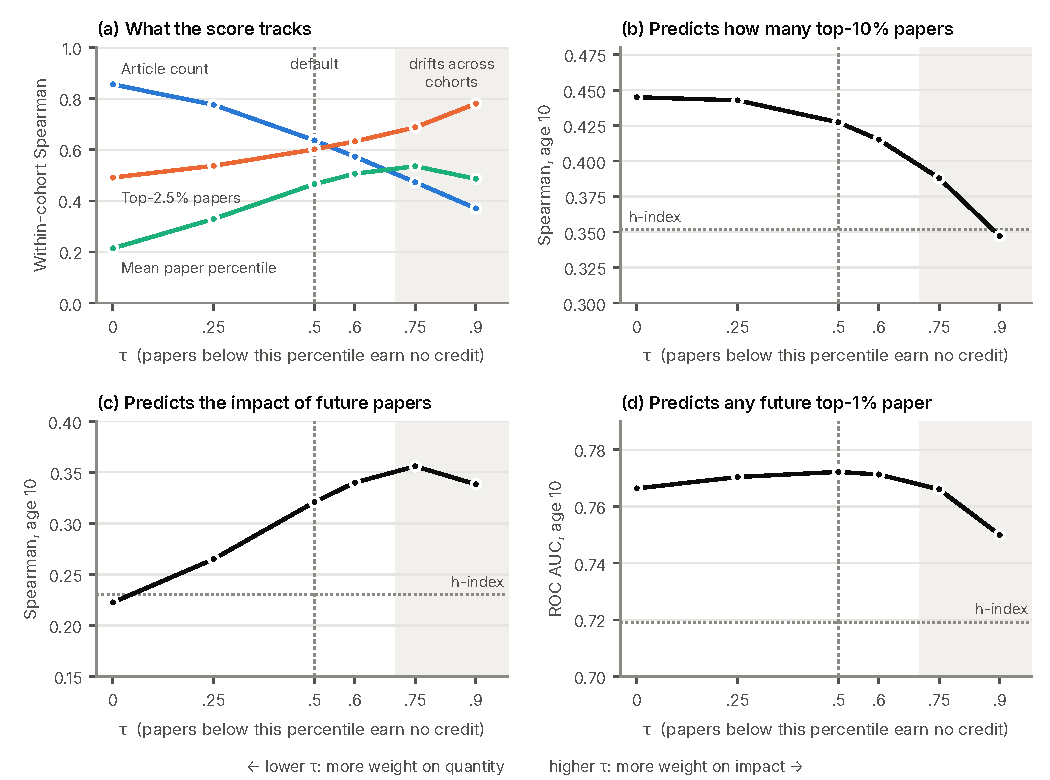
\includegraphics[width=\textwidth]{tau_sweep.pdf}
  \caption{The cutoff $\tau$ moves PiP from quantity towards impact. Eligible authors at career age 10, start years
  1975--2010. (a) Within-cohort Spearman correlation of PiP with the author's number of articles, number of articles in
  the top 2.5\% of their year, and mean article percentile. (b--d) Prediction of the author's articles published in the
  next ten years, for start years 1975--2000 (Section~\ref{sec:prediction}): (b) Spearman correlation with the number of
  future top-10\% articles, (c) Spearman correlation with their mean percentile, (d) ROC AUC for publishing at least one
  top-1\% article. The horizontal line shows the $h$-index. In the shaded range the score's distribution drifts across
  cohorts.}
  \label{fig:tau}
\end{figure}

\begin{table}[t]
  \centering
  \footnotesize
  \setlength{\tabcolsep}{4.5pt}
  \begin{threeparttable}
  \caption{PiP at different cutoffs $\tau$, career age 10. Columns 2--4: within-cohort Spearman correlation with
  characteristics of the record (3.43 million authors, start years 1975--2010). Columns 5--7: prediction of the next
  ten years (1.45 million authors, start years 1975--2000). Last column: median score of the 1960 and 2010 cohorts.}
  \label{tab:tau}
  \begin{tabular}{lccccccc}
    \toprule
    & \multicolumn{3}{c}{Correlation with} & \multicolumn{3}{c}{Prediction} & \\
    \cmidrule(lr){2-4}\cmidrule(lr){5-7}
    $\tau$ & Articles & Mean pct. & Top 2.5\% & Top-10\% count & Top-1\% AUC & Mean pct. & Median \\
    \midrule
    0 & 0.856 & 0.214 & 0.491 & \textbf{0.445} & 0.766 & 0.223 & 0.44 $\to$ 0.40 \\
    0.25 & 0.776 & 0.329 & 0.537 & 0.443 & 0.770 & 0.265 & 0.43 $\to$ 0.39 \\
    \textbf{0.5} & 0.637 & 0.466 & 0.602 & 0.427 & \textbf{0.772} & 0.321 & 0.41 $\to$ 0.38 \\
    0.6 & 0.573 & 0.506 & 0.633 & 0.415 & 0.771 & 0.340 & 0.41 $\to$ 0.37 \\
    0.75 & 0.473 & \textbf{0.536} & 0.688 & 0.388 & 0.766 & \textbf{0.356} & 0.38 $\to$ 0.33 \\
    0.9 & 0.370 & 0.486 & \textbf{0.781} & 0.347 & 0.750 & 0.338 & 0.37 $\to$ 0.16 \\
    \midrule
    $h$-index & -- & -- & -- & 0.352 & 0.719 & 0.230 & -- \\
    \bottomrule
  \end{tabular}
  \end{threeparttable}
\end{table}

As $\tau$ rises, the correlation with the number of articles falls from 0.86 to 0.37, that with the number of
top-2.5\% articles rises from 0.49 to 0.78 and that with the mean percentile peaks at $\tau = 0.75$. The same dial
trades quantity for impact when PiP predicts the author's future articles (Section~\ref{sec:prediction}): the
\emph{number} of future top-10\% papers is best predicted at low $\tau$, and the \emph{citation impact} of future
articles (their mean percentile) at $\tau = 0.75$; the chance of a future top-1\% paper is predicted about equally well
from $\tau = 0.25$ to $0.6$.

Above $\tau = 0.6$ the score's distribution drifts across cohorts. The drift comes from ties at zero
(Eq.~\ref{eq:mean}): the share of eligible authors with no article in the top 10\% of its year rises from 6\% to 42\%
between the 1960 and 2010 cohorts, and all of them score zero at $\tau = 0.9$.

We use $\tau = 0.5$ as the default: it has a one-line explanation (only papers in the top half of their year count),
balances the correlations with quantity (0.64) and with top papers (0.60), best predicts a future top-1\% paper and
keeps the score's distribution stable across cohorts. Users who favor volume can lower it, and those who favor impact
can raise it up to about 0.6; the choice should be made before the evaluation and stated.

\paragraph{Retrospective temporal robustness check.} The default was chosen from results that pooled all cohorts, so we
checked afterwards whether the choice depends on which cohorts it is made from. Because the check was made after the
default was chosen, it does not protect against specification search as an untouched holdout would. We split the
prediction settings that compare authors of one career age into a choice sample (start years 1975--1990) and a test
sample (start years 1991 and later). Stated as a rule, the default is the cutoff with the highest AUC for a future
top-1\% paper among cutoffs whose distribution is stable across cohorts ($\tau \le 0.6$). Applied to the choice sample
alone, the rule selects $\tau = 0.6$ at career age 10, with $\tau = 0.5$ within 0.001. The choice cohorts differ from
the test cohorts in two respects. The knee of their quantity--impact frontier (Figure~\ref{fig:frontier}) lies at a
slightly higher cutoff (between 0.6 and 0.75 rather than at 0.5). In those cohorts at career age 5, the top-10\% count
ties $\tau = 0.5$ on the top-1\% outcome and beats it on future citation impact, whereas $\tau = 0.6$ keeps its lead.

In the test cohorts both cutoffs keep every comparison reported in Sections~\ref{sec:prediction}--\ref{sec:early} at
career ages 5, 10 and 15: they beat the $h$-index on all three outcomes, no other indicator beats either of them on more
than one outcome, and both have the highest AUC for a future top-1\% paper. Across $\tau$ from 0.25 to 0.6 that AUC
varies by less than 0.01 in the test cohorts, so the exact choice in this range matters little for that outcome.

\subsection{The distribution of PiP is stable across cohorts}
\label{sec:cohorts}

Committees compare people who started in different years, and indicators are often read against fixed rules of thumb.
A fixed rule treats every start year alike only if the indicator's distribution does not change with the start year.
Figure~\ref{fig:cohorts} shows the distributions of PiP and the raw $h$-index at career age 10 for every start year
from 1960 to 2015. The cohorts grow nearly a hundredfold, from 4,031 eligible authors in 1960 to 392,360 in 2015. The
PiP distribution changes little: the mean goes from 0.44 to 0.42, the lower quartile from 0.20 to 0.16, the upper
quartile stays at 0.66--0.67 and the 90th percentile at 0.85. Over the same cohorts the mean $h$-index at age 10 rises
by 40\%, from 4.4 in the 1960 cohort to 6.2 in 2010 (6.1 in 2015), and its 90th percentile from 7 to 11, following the
growth of publication and citation rates.

\begin{figure}[t]
  \centering
  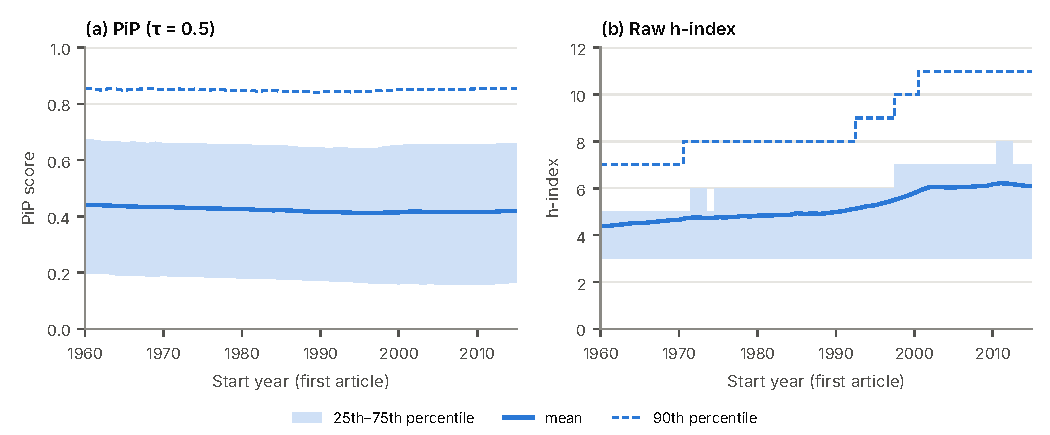
\includegraphics[width=\textwidth]{fig_cohorts.pdf}
  \caption{Distribution of (a) PiP ($\tau = 0.5$) and (b) the raw $h$-index of eligible authors at career age 10, by
  start year. The PiP distribution changes little over 56 cohorts; the mean $h$-index grows by about 40\%.}
  \label{fig:cohorts}
\end{figure}

Part of this stability is built in. The standing counts peers with strictly fewer articles, so a tie earns neither peer
credit, whereas two random peers who do not tie are equally likely to be ahead. The mean score of a peer group is
therefore one half minus half the probability that two random peers tie at a random threshold above $\tau$
(Eq.~\ref{eq:mean}), so it can move only as far as ties change. The rest of the distribution is not fixed by
construction: it drifts where ties at zero become common (above $\tau = 0.6$, Section~\ref{sec:tau}).

The stability establishes only rarity: a PiP of 0.6 at age 10 was about equally rare in the 1970 and 2010 cohorts, so
scores at the same career age can be read as statements of rarity, whatever the start year. A cohort percentile of the
$h$-index offers the same kind of scale. Stable rarity does not by itself mean that equal scores predict equal futures
across cohorts; Section~\ref{sec:prediction} tests prediction on pooled cohorts and seniorities.

\subsection{Stability over a career}
\label{sec:careerstability}

An indicator that reshuffles scholars every few years is of little use for decisions with long consequences. To measure
this reshuffling, we correlate each indicator's within-cohort percentile at two career ages, for authors who started in
1975--1995 (Table~\ref{tab:careerstability}). Over horizons starting early in a career, PiP is much more stable than
the $h$-index: between ages 5 and 30 its correlation is 0.56, against 0.37 for the $h$-index and 0.45 for citations.
The $h$-index is particularly unstable early on, partly because many eligible authors share the values 3 and 4.
Citations are slightly more stable than PiP between ages 5 and 10 and less stable over longer horizons. The article
count alone is more stable than PiP at every horizon, as expected of a quantity that only accumulates.

\begin{table}[t]
  \centering
  \small
  \caption{Stability of scholar indicators over a career. Correlation between an indicator's within-cohort percentile
  at two career ages (equal to the Spearman correlation of the raw values within cohort); eligible authors with start
  years 1975--1995. The 5-vs-30 comparison covers 434,000 authors.}
  \label{tab:careerstability}
  \begin{tabular}{lccccc}
    \toprule
    Indicator & 5 vs.\ 10 & 5 vs.\ 15 & 5 vs.\ 30 & 10 vs.\ 30 & 20 vs.\ 30 \\
    \midrule
    Articles & 0.847 & 0.754 & 0.642 & 0.800 & 0.946 \\
    \textbf{PiP} ($\tau = 0.5$) & 0.781 & 0.687 & 0.563 & 0.726 & 0.911 \\
    Citations & 0.798 & 0.659 & 0.451 & 0.620 & 0.886 \\
    $h$-index & 0.604 & 0.496 & 0.370 & 0.599 & 0.877 \\
    \bottomrule
  \end{tabular}
\end{table}
\subsection{Predicting future work}
\label{sec:prediction}

The hardest test of an indicator for career decisions is whether it anticipates the scholar's next work. For each
eligible author at evaluation year $Y$, we score each article they publish in years $Y+1$ to $Y+10$ by its percentile
within its publication year at its own age 5 (at age 5 a paper's percentile already correlates at 0.96 with its age-10
percentile; Section~\ref{sec:paperstability}). Indicators use only the author's articles and citations up to the
evaluation year, so no article counts towards both predictor and outcome. We use three outcomes, each with its own
accuracy measure: the number of future articles in the top 10\% (Spearman correlation); whether at least one future
article is in the top 1\% (ROC AUC: here and below, the probability that a random author with the outcome outranks a
random author without it, counting ties as one half, so 0.5 is chance); and the citation impact of the future
articles, defined as their mean percentile, among authors with at least one (Spearman correlation). We compare PiP with
the $h$-index, total citations, the article count and several indicators built from the same paper percentiles
(defined below).

Spearman correlation and ROC AUC both depend only on how an indicator orders people. Within one cohort a raw indicator
and its cohort percentile order people identically, so we pool cohorts in two ways that give five settings.
\emph{Same career age} (as for a tenure committee comparing candidates of similar seniority): all eligible authors at
career age $A = 5$, 10 or 15, with start years 1975 to $2010 - A$, so that every future article has five years of
citations by 2025 (start years 1975--2000 at career age 10). \emph{Same year} (as for a panel comparing people of
different seniority): all eligible authors in 2000 or 2005, at career ages 2 to 30. Across start years, an indicator's
raw and percentile forms no longer rank people identically, so in the same-year settings we compare each indicator in
both forms.

\begin{figure}[t]
  \centering
  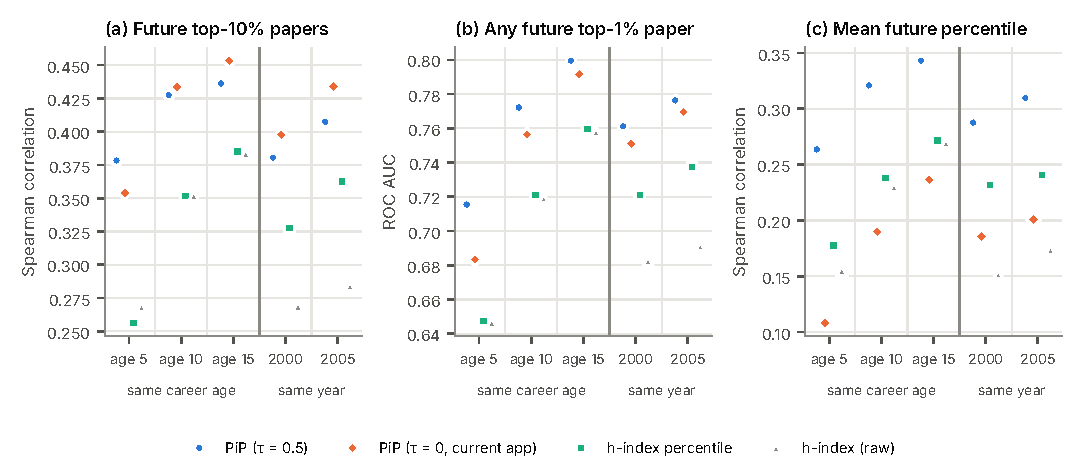
\includegraphics[width=\textwidth]{fig_prediction.pdf}
  \caption{Prediction of the next ten years of a scholar's work from indicators at the evaluation year. Settings:
  eligible authors at career age 5, 10 or 15 (left of the vertical line), or all eligible authors in 2000 or 2005 at
  career ages 2--30 (right). Outcomes: (a) Spearman correlation with the number of future articles in the top 10\% of
  their year; (b) ROC AUC for at least one future top-1\% article; (c) Spearman correlation with the mean percentile
  of future articles. Each future article is scored at age 5. Grey segments join PiP to the cohort percentile of the
  $h$-index.}
  \label{fig:prediction}
\end{figure}

\begin{table}[t]
  \centering
  \small
  \begin{threeparttable}
  \caption{Prediction of the next ten years of work. Career age 10 (1.45 million authors, start years 1975--2000; raw
  values, pooled over start years) and all eligible authors in 2005 (1.85 million authors, career ages 2--30;
  within-cohort percentiles, except where noted). Spearman correlation with the number of future top-10\% articles, ROC
  AUC for at least one future top-1\% article, and Spearman correlation with the mean percentile of future articles. The
  best value in each column is in bold. PiP-simple (Section~\ref{sec:definition}) compares the scholar with peers only
  once.}
  \label{tab:prediction}
  \begin{tabular}{lcccccc}
    \toprule
    & \multicolumn{3}{c}{Career age 10, raw} & \multicolumn{3}{c}{Year 2005, cohort pct.} \\
    \cmidrule(lr){2-4}\cmidrule(lr){5-7}
    Indicator & Top-10\% & Top-1\% & Mean pct. & Top-10\% & Top-1\% & Mean pct. \\
    \midrule
    \textbf{PiP} ($\tau = 0.5$) & 0.427 & \textbf{0.772} & 0.321 & 0.416 & \textbf{0.781} & 0.318 \\
    \quad PiP-simple ($\tau = 0.5$) & 0.430 & 0.765 & 0.296 & 0.422 & 0.778 & 0.296 \\
    \addlinespace
    $h$-index & 0.352 & 0.719 & 0.230 & 0.363 & 0.737 & 0.241 \\
    \quad raw, in 2005 & & & & 0.284 & 0.691 & 0.174 \\
    Citations & 0.290 & 0.714 & 0.298 & 0.312 & 0.733 & 0.303 \\
    Articles & 0.437 & 0.740 & 0.000 & \textbf{0.439} & 0.757 & 0.019 \\
    \addlinespace
    Top-10\% count & 0.360 & 0.748 & 0.338 & 0.354 & 0.762 & 0.324 \\
    \quad per year of career, raw & & & & 0.379 & 0.771 & 0.345 \\
    Top-1\% count & 0.250 & 0.641 & 0.228 & 0.262 & 0.698 & 0.225 \\
    I3 (sum of percentiles) & \textbf{0.438} & 0.755 & 0.182 & 0.434 & 0.769 & 0.189 \\
    Mean percentile & $-0.043$ & 0.523 & \textbf{0.394} & $-0.042$ & 0.526 & \textbf{0.404} \\
    \bottomrule
  \end{tabular}
  \end{threeparttable}
\end{table}

PiP beats the $h$-index on all three outcomes, in all five settings (Figure~\ref{fig:prediction},
Table~\ref{tab:prediction}). At career age 10, its correlation with the number of future top-10\% papers is 0.43 against
0.35, its AUC for a future top-1\% paper 0.77 against 0.72, and its correlation with future citation impact 0.32
against 0.23. The gap is larger when seniority differs: in 2005 the raw $h$-index reaches 0.28, 0.69 and 0.17, against
0.41, 0.78 and 0.31 for raw PiP. Converting the $h$-index into a cohort percentile helps (0.36, 0.74, 0.24) but does
not close the gap. PiP gains much less from conversion: in 2005 its cohort percentile reaches 0.42, 0.78 and 0.32,
because the raw score is already relative to the cohort and its distribution varies little across start-year cohorts
at a given career age (Section~\ref{sec:cohorts}). We report cohort percentiles for every indicator in the same-year
settings. In the same-career-age settings the two forms nearly agree; Table~\ref{tab:predictionall} in the appendix
gives raw PiP and both $h$-index forms in all five settings and under the three-article rule.

\paragraph{Productivity and citations.} Because productive authors keep producing, the article count predicts the
number of future top-10\% papers as well as PiP or slightly better (0.44 against 0.43 at age 10), but not future
citation impact (correlation 0.00). Total citations predict future citation impact about as well as PiP (0.30 against
0.32) but are weaker on the number of future top papers (0.29).

\paragraph{Percentile-based indicators.} The closest alternatives to PiP combine the same paper percentiles differently:
the number of papers in the top 10\% \citep{waltman2012leiden}, also divided by career age
\citep{bornmann2014individual}; the number in the top 1\%; I3, the sum of the percentiles
\citep{leydesdorff2011integrated}; and their mean. Apart from the top-1\% count, which trails PiP on all three outcomes,
each is best or nearly best on one outcome and weak on another (Table~\ref{tab:prediction}). The mean percentile
predicts future citation impact best (0.39 at age 10, against 0.32 for PiP), but says nothing about how many top papers
will follow ($-0.04$) or whether one will be in the top 1\% (AUC 0.52). I3 predicts the number of future top papers as
well as the article count does (0.44) but not their citation impact (0.18). The top-10\% count predicts future citation
impact slightly better than PiP (0.34 against 0.32) and the number of future top papers clearly worse (0.36 against
0.43). In all five settings, each of these indicators beats PiP on at most one of the three outcomes, and none on the
chance of a future top-1\% paper. PiP predicts a future top-1\% paper best in every setting. Of these indicators, the
top-10\% count, I3 and the mean percentile each serve one outcome, whereas PiP balances all three.

\begin{figure}[t]
  \centering
  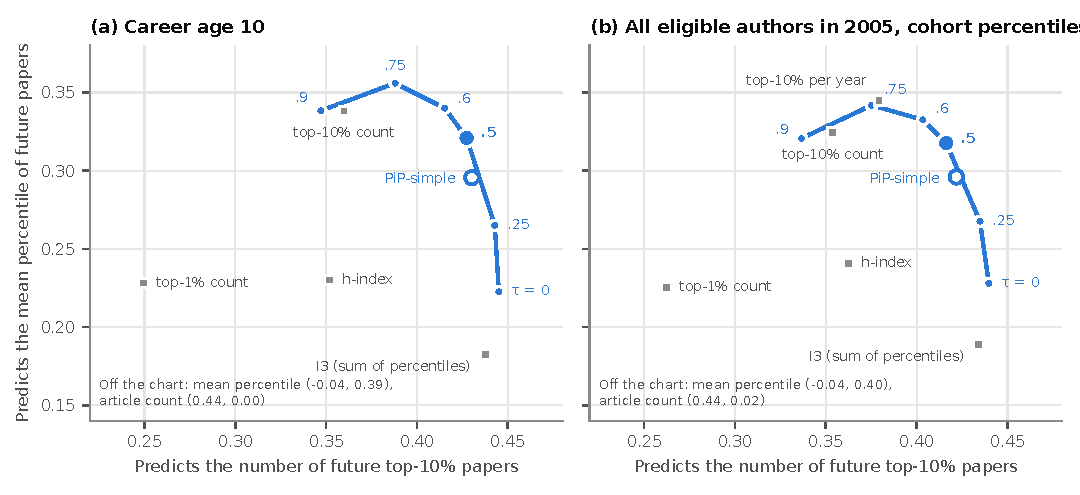
\includegraphics[width=\textwidth]{fig_frontier.pdf}
  \caption{Indicators placed by how well they predict the number of a scholar's future top-10\% papers (horizontal) and
  the mean percentile of their future papers (vertical), Spearman correlations. The blue curve is PiP at cutoffs from
  $\tau = 0$ to $0.9$; the large dot is $\tau = 0.5$. Grey squares are the $h$-index, I3, the top-10\% and top-1\%
  counts and, in panel (b), the top-10\% count per year of career; the mean percentile and the article count lie off
  the chart, and their coordinates are printed in each panel. (a) Eligible authors at career age 10, raw values. (b) All
  eligible authors in 2005 at career ages 2--30, within-cohort percentiles (the top-10\% count per year of career is
  raw). The open circle is PiP-simple ($\tau = 0.5$), which compares the scholar with peers only once. For the third
  outcome, a future top-1\% paper, PiP at every cutoff from 0 to 0.75 has a higher AUC than every
  grey indicator in both settings.}
  \label{fig:frontier}
\end{figure}

Across its cutoffs, PiP traces a frontier for two outcomes, the number of future top papers (quantity) and future
citation impact (Figure~\ref{fig:frontier}). Its curve lies on or outside the other ways of combining paper percentiles,
apart from two extremes, the mean percentile and the article count. With $\tau = 0$, PiP predicts at least as well as I3
on all three outcomes in every setting (with $\tau = 0.25$, in all but one); with $\tau = 0.75$ it does at least as well
as the top-10\% count on all three outcomes in every setting; and from $\tau = 0.25$ to $0.75$ it does better than the
$h$-index on all three. Three indicators lie on or beyond the frontier. The mean percentile lies beyond it in the
direction of pure citation impact, where it gives up any information about quantity. The article count lies just beyond
it in two settings (at age 15 and in 2000), in the direction of pure quantity. The top-10\% count per year of career
differs from the plain count only when seniorities are mixed, and it lies on the curve next to $\tau = 0.75$. The cutoff
therefore selects a point on the frontier, and $\tau = 0.5$ sits near its knee: from $\tau = 0.25$ to $0.5$ the curve
gains 0.056 in future citation impact for 0.016 in quantity, and beyond $0.5$ each gain in impact costs more in
quantity.

\paragraph{Replication across cohorts.} With more than a million authors per setting, sampling error is small: the
standard error of a Spearman correlation of 0.4 would be below 0.001 for independent observations. Authors share
papers, so the observations are not independent and this standard error is optimistic. The more relevant question is
whether the differences hold in different populations. We repeated the age-10 comparison separately for each start
year from 1975 to 2000, 26 cohorts of 17,867 to 122,114 authors. PiP beats the $h$-index on all three outcomes in all
26 cohorts, by 0.06--0.10 on the number of future top papers. It beats the top-10\% count on the number of future top
papers (by 0.05--0.08) and on the top-1\% outcome in all 26 cohorts, and falls behind it on future citation impact in
20 (by up to 0.07). Against I3 and the article count, PiP wins on the top-1\% outcome and on future citation impact in
every cohort, and on the number of future top papers in 12 and 11 of the 26, with differences between $-0.03$ and
$+0.04$.

\paragraph{Comparing with peers at every threshold.} PiP-simple (Section~\ref{sec:definition}) uses the same percentiles
and cutoff as PiP but compares the scholar with peers only once, through the rank of its score in the cohort. The pair
therefore shows what the comparison at every threshold contributes. In each of the 26 cohorts at career age 10, that
comparison improves the AUC for a future top-1\% paper (by 0.004 to 0.011) and the prediction of future citation impact
(by 0.023 to 0.036); the same holds in every cohort at career ages 5 and 15. On the number of future top-10\% papers PiP
and PiP-simple are within 0.01 of each other.

\subsection{Early detection}
\label{sec:early}

Early detection asks how soon each indicator picks out the scholars who will do well later. We therefore fix the
population and the outcome and vary only the measurement age. The population is every author eligible at career age 3
(306,854 authors, start years 1975--2000); because eligibility persists, each has every indicator at every later age.
The outcome is their work at career ages 11--20, scored as before (each article at its own age 5). A \emph{future star},
or future high performer, is an author in the top 10\% of their start-year cohort, within the population, by the number
of top-10\% articles at ages 11--20 (ties broken by the articles' mean percentile).

We measure each indicator at career ages 3, 4, \ldots, 10 as a cohort percentile and ask how well it finds future
stars. The first measure is precision: the share of future stars among the top 10\% of each cohort by the indicator
(chance is 0.10). Authors tied at the boundary of the top 10\% (common on the $h$-index) each count with the share of
the remaining places, which gives the expected precision under random tie-breaking. The second is the AUC for future
stars, and the third the AUC for at least one top-1\% article at ages 11--20.

\begin{figure}[t]
  \centering
  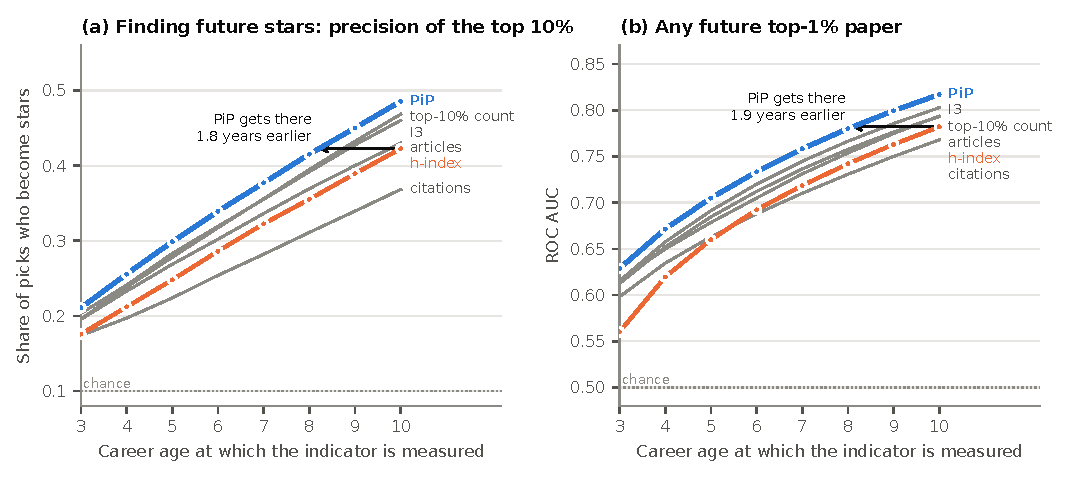
\includegraphics[width=\textwidth]{fig_early.pdf}
  \caption{Early detection. Authors eligible at career age 3 (306,854; start years 1975--2000), with each indicator
  measured at career ages 3 to 10 and the outcome fixed: their articles published at career ages 11--20. (a) Of the
  authors in the top 10\% of their cohort by the indicator (ties at the boundary shared at random), the share who
  become future stars (the top 10\% of the cohort by the number of top-10\% articles at ages 11--20). (b) ROC AUC for
  at least one top-1\% article at ages 11--20. The arrow marks the career age at which PiP reaches the accuracy that the
  $h$-index has at age 10.}
  \label{fig:early}
\end{figure}

\begin{table}[t]
  \centering
  \small
  \caption{How much earlier PiP reaches each indicator's accuracy, in years. For each target age $T$ from 5 to 10, we
  find the (interpolated) age at which PiP first matches the indicator's accuracy at $T$; the table gives the range of
  $T$ minus that age. Authors eligible at career age 3, outcome at career ages 11--20.}
  \label{tab:early}
  \begin{tabular}{lccc}
    \toprule
    Compared with & Precision for future stars & AUC for future stars & AUC for a future top-1\% paper \\
    \midrule
    Citations & 1.7--3.2 & 1.4--2.8 & 1.2--2.6 \\
    $h$-index & 1.2--1.8 & 1.1--1.6 & 1.3--1.9 \\
    Articles & 0.7--1.6 & 0.3--0.9 & 0.6--1.3 \\
    Top-10\% count & 0.5--0.6 & 1.0--1.3 & 0.8--1.3 \\
    I3 & 0.4--0.7 & 0.2--0.4 & 0.4--0.8 \\
    \bottomrule
  \end{tabular}
\end{table}

PiP is the most accurate indicator at every measurement age on all three measures (Figure~\ref{fig:early} shows
precision and the AUC for a future top-1\% paper; Table~\ref{tab:early}, lead times on all three). At career age 3,
the top 10\% of a cohort by PiP contains 21\% future stars, twice the chance rate, against 18\% for the $h$-index; at
age 5 the shares are 30\% and 25\%, and at age 10, 49\% and 42\%. The AUC for a future top-1\% paper is 0.63 against
0.56 at age 3 and 0.71 against 0.66 at age 5.

Because every indicator improves with age, the gaps translate into time (Table~\ref{tab:early}): across the three
measures, PiP reaches the $h$-index's age-10 accuracy 1.6 to 1.9 years earlier (1.6 to 1.8 on the two measures for
future stars), at about age 8, and the citation count's 2.6 to 3.2 years earlier. Its lead over the article count, the
top-10\% count and I3 is smaller, at most 1.6 years. For the 711,986 authors eligible at age 5, PiP reaches
the $h$-index's age-10 accuracy 1.5 to 1.8 years earlier and the citation count's 2.3 to 2.9 years earlier.

\paragraph{Without the h-index condition.} Requiring an $h$-index of three by career age 3 keeps only 21\% of the
authors who have three articles by then, and it selects the population by one of the indicators being compared. We
therefore repeated it for all 1,455,891 authors with at least three articles at career age 3, with peers defined by the
same rule. PiP still leads the $h$-index at every measurement age: the top 10\% by PiP contains 24\% future stars at age
3 against 20\% for the $h$-index, and 31\% against 27\% at age 5. PiP reaches the $h$-index's age-10 accuracy 1.2 to 1.7
years earlier. It also leads the indicators of Table~\ref{tab:early} on precision and the AUC for a future top-1\% paper
at every age, but I3 matches or beats it on the AUC for future stars from about age 6.

On the other two outcomes the ordering at each age matches that of Section~\ref{sec:prediction}: the article count
predicts the number of future top-10\% papers slightly better than PiP at the earliest ages, and the mean percentile
predicts future citation impact best. PiP's early-detection advantage lies in finding the scholars at the top, who
combine many papers with highly cited ones, and in anticipating exceptional papers. PiP-simple is about as accurate
here: within 0.007 of PiP at every age, in every population we tested, and within 0.3 years in lead time; under the
three-article rule it is slightly ahead on finding future stars from career age 6 or 7. In early detection the gain over
the $h$-index therefore comes mainly from what PiP and PiP-simple share: percentiles within the publication year and the
cutoff.
\subsection{Later recognition}
\label{sec:honors}

So far we have judged citation indicators by later citations; as a check, we ask whether the indicators anticipate an
outcome that is not a citation count: later scientific honors. From Wikidata (Section~\ref{sec:data}) we take 65 senior
honors for research: membership of national academies (such as the US National Academy of Sciences, the Royal Society
and the Leopoldina); fellowships of learned societies (AAAS, ACM, IEEE, APS and others); and major prizes and
fellowships (such as the Guggenheim, MacArthur and Gairdner awards). We exclude plain society memberships, state orders,
student scholarships and the citation-based Clarivate Citation Laureates. We connect honors to Semantic Scholar authors
in two ways: through Wikidata items with a Semantic Scholar author ID (41,272 items, honored or not), and through items
with a Google Scholar ID (12,434 honorees), linked to Semantic Scholar by title matching (Section~\ref{sec:robustness}).

We measure each indicator at career age 5 or 10 as a percentile within the start-year cohort (start years 1960--2000).
So that every counted honor follows the evaluation, the main analysis uses only dated honors: we drop people whose
first dated honor came at or before that age or whose honors are all undated. Most honors come decades later. This
leaves 919 future honorees at age 5 and 1,308 at age 10. The ROC AUC measures how well each indicator's ranking
separates future honorees from the others, among all eligible authors and within two already notable groups: people
with a Wikidata item, and our Google Scholar profiles matched to Semantic Scholar (mostly faculty).

\begin{table}[t]
  \centering
  \small
  \caption{ROC AUC for holding a senior honor. Columns 2--5: indicators measured at career age 5 or 10 in Semantic
  Scholar against dated honors received later, among all eligible authors (the comparison uses every honoree and a 10\%
  random sample of the others: 919 future honorees among 78,431 sampled authors at age 5, and 1,308 among 161,609 at
  age 10), among people with a Wikidata item, and among our Google Scholar profiles matched to
  Semantic Scholar (mostly faculty; GS: Google Scholar). Columns 6--7: current Google Scholar scores of the 15,890
  profiled scholars who meet the eligibility rule and belong to a start-year cohort of at least 30 profiles, against
  holding an honor and having an English Wikipedia article (agreement, not prediction). PiP's bootstrap intervals are
  about $\pm 0.015$ for all authors and $\pm 0.025$ within the smaller groups; differences between indicators are
  estimated more precisely because they are paired.}
  \label{tab:honors}
  \setlength{\tabcolsep}{4.5pt}
  \begin{tabular}{lcccccc}
    \toprule
    & \multicolumn{4}{c}{Predicting later honors (Semantic Scholar)} & \multicolumn{2}{c}{Google Scholar, now} \\
    \cmidrule(lr){2-5}\cmidrule(lr){6-7}
    & All, age 5 & All, age 10 & Wikidata, 10 & GS faculty, 10 & Honors & Wikipedia \\
    Future honorees / positives & 919 & 1,308 & 629 & 755 & 1,497 & 2,160 \\
    \midrule
    \textbf{PiP} ($\tau = 0.5$) & 0.751 & 0.827 & 0.641 & 0.648 & 0.712 & 0.716 \\
    PiP ($\tau = 0.75$) & \textbf{0.761} & \textbf{0.836} & \textbf{0.658} & \textbf{0.654} & 0.711 & \textbf{0.721} \\
    $h$-index & 0.709 & 0.790 & 0.618 & 0.637 & 0.708 & 0.704 \\
    Citations & 0.700 & 0.798 & 0.637 & 0.638 & \textbf{0.714} & \textbf{0.721} \\
    Articles & 0.694 & 0.783 & 0.579 & 0.628 & 0.677 & 0.675 \\
    Top-10\% count & 0.748 & 0.826 & 0.656 & 0.649 & 0.709 & 0.720 \\
    I3 & 0.722 & 0.799 & 0.607 & 0.639 & 0.696 & 0.692 \\
    Mean percentile & 0.531 & 0.572 & 0.574 & 0.541 & 0.611 & 0.611 \\
    \bottomrule
  \end{tabular}
\end{table}

Among all eligible authors, PiP at career age 5 reaches an AUC of 0.75, against 0.71 for the $h$-index and 0.70 for
citations; at age 10, 0.83 against 0.79 and 0.80 (Table~\ref{tab:honors}). Paired bootstrap intervals for PiP's lead
over the $h$-index exclude zero at both ages ($+0.042$ [0.031, 0.052] and $+0.037$ [0.031, 0.043]). PiP ties the
top-10\% count ($+0.001$ [$-0.005$, 0.007] at age 10), and the impact end of the dial beats the default: at
$\tau = 0.75$ the AUC is 0.76 and 0.84. Recognition rewards highly cited work more than volume: the article count,
which leans most towards volume, does worst apart from the mean percentile.

Within the two notable groups, every indicator separates future honorees only weakly (AUC 0.54--0.66 at career age
10). There, PiP is level with the $h$-index at age 5 ($-0.005$ [$-0.019$, 0.011] among people with a Wikidata item and
$+0.001$ [$-0.011$, 0.013] among the Google Scholar faculty; not in the table) and ahead at age 10, by 0.022 [0.014,
0.030] and 0.011 [0.005, 0.018]. The top-10\% count and PiP at $\tau = 0.75$ or higher do best. Counting undated
honors as later (1,064 honorees at age 5 and 1,555 at age 10) changes little: PiP's AUC is 0.75 against 0.71 for the
$h$-index at age 5, and 0.82 against 0.78 at age 10.

A last check measures agreement rather than prediction (columns 6--7 of Table~\ref{tab:honors}). On the Google Scholar
profiles, where scores and honors are measured at the same time, the indicators are close: PiP is slightly ahead of the
$h$-index for holding an honor ($+0.004$ [0.001, 0.008]) and for having a Wikipedia article ($+0.012$ [0.009, 0.015]).
Total citations and the top-10\% count do as well for holding an honor (their paired differences from PiP include zero)
and slightly better for having a Wikipedia article (by 0.005 and 0.004).

The recognition test therefore supports PiP over the $h$-index with an outcome outside citation counts, most clearly for
detecting future honorees among all scholars and early in their careers. In populations closer to faculty evaluation,
the gain over the $h$-index is small, and the top-10\% count does as well. The test also shows that the default cutoff
is not best for every purpose: to anticipate recognition, an evaluator should move the dial towards impact. Above $\tau
= 0.6$ the raw score drifts across cohorts (Section~\ref{sec:tau}), so such scores should be read as cohort percentiles,
as they are here.

Several caveats apply. Wikidata covers honors unevenly across countries and fields, so an author without a recorded
honor is not a confirmed non-recipient; older cohorts have had more time to receive senior honors; and honors depend
on nominations, networks and opportunity as well as on the work. These processes can strengthen or weaken an
indicator's association with recorded honors, so the AUCs measure agreement with recorded recognition, not with merit.

\subsection{Fields}
\label{sec:fields}

The main analysis pools fields: it ranks each paper against all articles from its year, although fields cite at
different rates. Two questions follow: whether PiP's lead holds within each field, and whether pooling favors some
fields. For the first, we assign each author a main field, the most frequent among their articles by career age 10
(an article with several fields counts in full for each), and repeat the analyses by field. Fifteen fields have at
least 3,000 eligible authors with start years 1975--2000. In every one, PiP predicts better than the $h$-index on all
three outcomes. For example, in economics PiP reaches 0.39 / 0.74 / 0.27 against 0.31 / 0.67 /
0.17 for the $h$-index, and in mathematics 0.38 / 0.75 / 0.28 against 0.29 / 0.68 / 0.19.

Pooled paper percentiles favor fields with high citation rates. A field-neutral score would put 10\% of each field's
authors in the top 10\% of their cohort; with pooled percentiles the share ranges from 1.4\% in education and 2.1\% in
economics to 14.7\% in physics (Figure~\ref{fig:fields}). We therefore also compute a field-normalized PiP. In this
version, each paper's percentile is computed within its publication year and the author's main field, and peers are
restricted to authors with the same main field and start year. A paper that does not carry the author's main field keeps
its pooled percentile. The rule also gives a coauthored paper different percentiles for coauthors with different main
fields, a choice that a rule based on the paper's own fields would avoid.

Among eligible authors at career age 10 with start years 1975--2010 (Figure~\ref{fig:fields}), the field-normalized
score puts every field's share of the cohort top 10\% between 6.9\% and 11.6\%. We have not separated the sources of the
remaining spread. Two candidates are that papers outside the author's main field keep their pooled percentile, and that
fields differ in how often peers tie, which also shapes the distribution of the score. Within a field the ranking
largely holds: pooled and field-normalized scores correlate at 0.91--0.99 per field.

\begin{figure}[t]
  \centering
  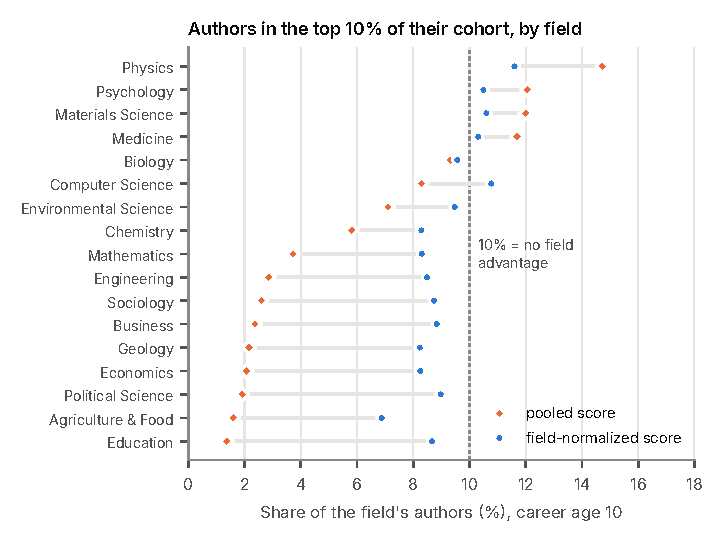
\includegraphics[width=0.72\textwidth]{fig_fields.pdf}
  \caption{Share of each field's authors who are in the top 10\% of their start-year cohort at career age 10, with
  PiP computed from pooled percentiles and with the field-normalized version. Eligible authors with start years
  1975--2010; fields with at least 5,000 such authors.}
  \label{fig:fields}
\end{figure}

The two versions answer different questions: how a scholar's future work will rank among all articles of its year,
and how it will rank within its field. With outcomes measured on pooled percentiles, the pooled score predicts
best (0.427 / 0.772 / 0.321 against 0.414 / 0.770 / 0.298); with field-normalized outcomes, the field-normalized score
predicts best (0.407 / 0.772 / 0.316 against 0.405 / 0.769 / 0.300). Both remain far ahead of the $h$-index
(0.333 / 0.717 / 0.209 on field-normalized outcomes). For comparisons across fields we recommend the field-normalized
version; within a field the two are nearly interchangeable.

\subsection{Robustness}
\label{sec:robustness}

\paragraph{Self-citations.} Part of an indicator's predictive power could run through authors citing their own work. A
citation counts as a self-citation when the citing and cited papers share at least one author. Self-citations are
8.1\% of all citations; such rates depend strongly on the definition and the citation window \citep{aksnes2003macro}.
We removed them and reran the whole pipeline (percentiles, the $h$-index condition for eligibility, peer groups,
scores and outcomes; Table~\ref{tab:selfcites} in the appendix). PiP's predictions of the number of future top-10\%
papers and of a future top-1\% paper move by at most 0.003. The $h$-index loses slightly more (0.352 to 0.340 at age
10). The prediction of future citation impact drops more, and unevenly: by 0.018 to 0.030 for PiP and by 0.005 to
0.009 for the $h$-index. PiP's lead on this outcome therefore shrinks but remains (0.298 against 0.221 at career age
10), and PiP stays ahead of the $h$-index on all three outcomes in every setting. Removing self-citations changes
paper percentiles, eligibility, peer groups and outcomes at once, so the drop does not isolate the effect of authors
citing their own work.

\paragraph{Eligibility without the h-index condition.} The main rule requires an $h$-index of three, which selects the
population by citations and by one of the compared indicators and excludes far more authors in some fields than in
others (Section~\ref{sec:data}). Under the three-article rule, the same-career-age settings grow to 2.81, 2.54 and
2.00 million authors at career ages 5, 10 and 15 (from 1.17, 1.45 and 1.24 million). PiP still beats the $h$-index on
all three outcomes at every age, by 0.03 to 0.06, half to two thirds of the margin under the main rule; at career age
10 it reaches 0.420, 0.805 and 0.493 against 0.376, 0.770 and 0.443 (Table~\ref{tab:predictionall}). Every indicator
predicts future citation impact better than under the main rule (the mean percentile 0.519 against 0.394, the article
count 0.163 against 0.000 at career age 10), as expected when the population spans a wider range of records: the added
authors lack three articles with three citations each. PiP again has the highest AUC for a future top-1\% paper, and
no other indicator beats it on more than one outcome. Section~\ref{sec:early} reports early detection under the same
rule.

\paragraph{Author disambiguation.} Semantic Scholar's author records come from automatic disambiguation, which can split
one person across several records or merge different people. To check that the results are not artifacts of this
algorithm, we use the author-curated Google Scholar profiles. We matched the 16,218 profiles to Semantic Scholar through
their publications. A profile's work matches a Semantic Scholar paper on its normalized title (at least 25 characters)
and a publication year within one year. The profile's counterpart is the Semantic Scholar author record with the same
surname that holds the most matched works. We find a confident counterpart (at least five matched works and at least
30\% of the profile's titles) for 14,511 profiles (89\%). For the median person, 76\% of their Google Scholar works are
found in Semantic Scholar, and 90\% of those found sit under the counterpart. Splitting is common, though: 64\% of
people have at least two of their works under a second record with the same surname and first initial, and 42\% under a
third. The counterpart is smaller than the profile (a median 67\% of the profile's cited works, and 78\% of its
$h$-index), and its start year is later than the profile's for 47\% of people, because early work is missing or sits
under another record.

Despite these differences, the two sources rank people similarly. For the 9,796 people who have scores in both sources
(Semantic Scholar start year 1995 or later, evaluated in 2025), the Spearman correlation between sources is 0.82 for the
$h$-index and 0.78 for PiP. Each source computes percentiles against its own population: all eligible Semantic Scholar
authors, and the Google Scholar profiles. For PiP, the agreement is lower for people split across three or more records
(0.73) than for people with at most one record (0.76), but not by much. We read these comparisons as evidence that the
results above are not artifacts of one disambiguation algorithm, and as a warning that individual Semantic Scholar
scores can be off when a person's work is split.

\paragraph{Survivorship.} The population includes every eligible author, not only those who stayed in research, and
the prediction results of Section~\ref{sec:prediction} count authors who stop publishing as having no future top
papers. This choice favors indicators that predict survival, that is, whether an author continues to publish. Measured
at career age 5, the indicators predict whether an author is still publishing at career ages 11--15 with an AUC of
0.68 for the article count, 0.62 for PiP, 0.58 for the $h$-index and 0.54 for citations. Continuing to publish is a
matter of volume, so the indicators that weigh volume most predict it best. PiP still leads the article count, the
best predictor of survival, on the top-1\% outcome and on future citation impact.
\section{Discussion}
\label{sec:discussion}

\paragraph{Why PiP improves on the $h$-index.} The $h$-index summarizes a record by one point; PiP uses every paper
above the cutoff, comparing the scholar with peers at every impact threshold. Three properties explain most of the
predictive gain. First, PiP credits the best papers in proportion to their rarity among peers: one top paper raises the
standing at the highest thresholds, where most peers have none. Second, PiP credits recent papers as soon as they pass
the cutoff among papers of the same age, whereas the $h$-index waits for enough raw citations. This credit matters most
early in a career, when most papers are recent, and likely explains much of PiP's lead in early detection
(Section~\ref{sec:early}). Third, PiP's scale does not depend on the start year: at the same career age, a given score
is about equally rare in every cohort (Section~\ref{sec:cohorts}), and in pools of mixed seniority the raw score
predicts almost as well as its cohort percentile (Section~\ref{sec:prediction}). The raw $h$-index instead favors longer
careers and later cohorts, which started when citation rates were higher.

Comparing PiP with PiP-simple shows what each part of PiP does. PiP-simple uses the same percentiles and cutoff, and so
shares the credit for recent papers, but compares the scholar with peers only once. Percentiles within the publication
year and the cutoff carry most of the gain over the $h$-index in predicting future top papers and in early detection,
where PiP-simple is about as early as PiP. The comparison at every threshold (the first property) adds the gain on
future citation impact and the chance of an exceptional paper.

\paragraph{Prediction and cumulative advantage.} Citations reward visibility as well as research quality: well-known
scholars attract more citations for comparable work \citep{merton1968matthew,petersen2014reputation}. For any
citation-based indicator, PiP and the $h$-index alike, part of the predictive power may therefore reflect reputation
feeding itself (cumulative advantage) rather than persistent research quality. The most mechanical channel of this
feedback is self-citation. Removing self-citations narrows PiP's lead on future citation impact but leaves it ahead of
the $h$-index on all three outcomes (Section~\ref{sec:robustness}). This check does not rule out the broader effect of
reputation; separating that effect from research quality would need variation in visibility unrelated to the work's
quality. Indicators can absorb cumulative advantage to different degrees, so it may also explain part of their
differences. The test against later honors (Section~\ref{sec:honors}) uses a non-citation outcome and gives the same
ordering of PiP and the $h$-index, although visibility also shapes honors.

\paragraph{Fields and windows.} The pooled score ranks each paper against all articles of its publication year,
whatever their field, and so favors high-citation fields; the field-normalized version removes most of that advantage.
Field normalization brings its own choices: the field scheme and the assignment of multi-field papers
\citep{zitt2005relativity,waltman2015field,waltman2019field} and, for a scholar, of a main field. Semantic Scholar's 23
fields are broad, and subfields with different citation habits share a reference set, so normalization removes only
differences between these broad fields.

Percentiles of recent papers are also noisier in slow-citing fields such as the humanities and law
(Section~\ref{sec:paperstability}), so in those fields PiP's credit for recent papers is least reliable and part of a
scholar's score rests on percentiles still settling. An evaluation there might count only papers older than two or
three years, at the cost of ignoring the most recent work.

\paragraph{Limitations.}
\begin{itemize}
  \item \emph{Disambiguation.} Semantic Scholar's automatic disambiguation can split one person's work across several
  author records or merge different people's work into one. Split records shorten careers and move start years,
  placing the person in a later cohort with a partial record. Evaluations of individuals should use a curated record
  such as a Google Scholar or ORCID profile.
  \item \emph{Whole counting.} Every coauthor receives full credit for every paper, whatever the number of authors or
  their roles. Compared with fractional counting, it favors authors in large teams. A fractional version would weight
  each paper's contribution to the author's count $n_a(\theta)$ at each threshold by the author's share
  \citep{waltman2015field}; we have not tested it.
  \item \emph{The peer group.} Peers share a start year, the year of the first article. Authors who start late,
  interrupt their careers or move between research and other work are compared with a cohort whose careers ran
  differently. The eligibility rule (three articles and an $h$-index of three) excludes much of the earliest career
  stage and of slow-citing fields; under the three-article rule the main comparisons hold with smaller margins
  (Sections~\ref{sec:early} and~\ref{sec:robustness}). Neither rule admits a scholar with one top paper and nothing else
  (Section~\ref{sec:properties}); such a record can be scored against a cohort, but our tests do not cover it.
  \item \emph{Retrospective reconstruction.} Publications and citations are counted up to each evaluation year, but
  author records, publication types and fields come from the 2026 release; an evaluation at the time would have seen
  different records.
  \item \emph{Reference set.} Each paper's reference set depends on Semantic Scholar's publication types, which are
  incomplete; untyped records are excluded from the reference sets, the paper counts and the $h$-index.
  \item \emph{Consistency.} Like the $h$-index, PiP is not consistent in the sense of \citet{waltman2012inconsistency}:
  adding the same article to two authors can reverse their order, though rarely in simulation.
\end{itemize}

\paragraph{Responsible use.} PiP is meant to inform comparisons among scholars at a similar career stage, alongside
reading the work itself and expert judgment, as the Leiden Manifesto \citep{hicks2015bibliometrics} and DORA
\citep{dora2012} recommend. Its cutoff should be chosen before an evaluation, not tuned to favor a candidate, and
comparisons across fields should use the field-normalized version. A predictive correlation of 0.4 leaves most of a
scholar's future unexplained.

\section{Conclusion}
\label{sec:conclusion}

PiP rates a scholar by the citation percentiles of their papers above a cutoff, comparing the scholar at every impact
threshold with peers who started in the same year. For 11.1 million Semantic Scholar authors, PiP's distribution changes
little across cohorts since 1960, and a scholar's PiP is more stable over a career than their $h$-index. PiP predicts
three outcomes better than the $h$-index in every setting and field we tested: the number of future top papers, the
chance of an exceptional paper and future citation impact. At the same career age, the lead narrows but remains when
eligibility does not depend on citations. No other indicator built from the same paper percentiles beats PiP on more
than one of them. PiP reaches the $h$-index's age-10 accuracy in detecting future high performers 1.6 to 1.8 years
earlier. PiP also anticipates later academy memberships, fellowships and prizes better than that index, though only
slightly within already notable groups. The results hold without self-citations, PiP rankings agree between Semantic
Scholar and author-curated Google Scholar profiles, and a field-normalized version removes most of the advantage of
high-citation fields.

A single parameter, the cutoff, moves PiP between quantity and impact. The construction needs only each scholar's
articles, with their publication years and citations by year. The website \url{https://www.pip-score.org} computes the
earlier form of the score, PiP-AUC (Section~\ref{sec:auc}), from Google Scholar profiles; the replication code
computes PiP itself at full scale in a database.
\section*{Data and code availability}
The replication package is the \texttt{paper/} directory of \url{https://github.com/ipeirotis-org/scholar_v2}. It holds
the SQL that builds every table in this paper, the result tables that the SQL writes, the numerical checks of the
properties in Section~\ref{sec:pip}, the data behind every figure, the plotting scripts, and the scripts and curated
honors of Section~\ref{sec:honors}. Its \texttt{COMPUTATION.md} explains how the SQL evaluates the integral that defines
PiP. Semantic Scholar data are available under the ODC-BY license from the Semantic Scholar Datasets API
\citep{s2datasets2026}; Wikidata is available under CC0 \citep{wikidata2026}. Author-level statistics for the Google
Scholar profiles can be downloaded from \url{https://www.pip-score.org/data}; the per-article profile data used here are
not redistributed. The derived tables, from the article-level reconstruction to the per-author scores, are in the
BigQuery datasets \texttt{scholar-version2.paper\_rp} and \texttt{scholar-version2.paper\_rp\_noself} (without
self-citations), which anyone signed in to Google Cloud can query; queries are billed to the reader's own project. The
result tables and a snapshot of the replication package are archived on Zenodo \citep{ipeirotis2026replication}.

\section*{Competing interests}
Panos Ipeirotis developed and maintains \url{https://www.pip-score.org}, a free, non-commercial website that computes
an earlier, asymmetric form of the score from Google Scholar profiles. The authors have no other competing interests.

\section*{Funding}
No specific funding was received for this work.

\section*{Author contributions}
Panos Ipeirotis: Conceptualization, Methodology, Software, Formal analysis, Data curation, Visualization, Supervision,
Writing -- original draft, Writing -- review \& editing. Sen Tian: Conceptualization, Methodology, Formal analysis,
Writing -- review \& editing.

\section*{Acknowledgments}
We thank the reviewers of an earlier version of this work for comments that shaped this one.

\bibliographystyle{apalike}
\bibliography{references}

\appendix
\section{Self-citations}
\label{app:selfcites}

\begin{table}[ht]
  \centering
  \small
  \caption{Prediction results with and without self-citations (with / without). Self-citations are removed
  throughout: in the paper percentiles, the peer groups, the scores and the outcomes. Raw scores, pooled over start
  years; for the year 2005, Table~\ref{tab:prediction} reports cohort percentiles, which differ slightly.}
  \label{tab:selfcites}
  \begin{tabular}{llccc}
    \toprule
    Setting & Indicator & Top-10\% count & Top-1\% AUC & Mean pct. \\
    \midrule
    Age 5 & PiP & .378 / .378 & .715 / .712 & .264 / .234 \\
          & $h$-index & .268 / .257 & .646 / .640 & .155 / .148 \\
    \addlinespace
    Age 10 & PiP & .427 / .427 & .772 / .771 & .321 / .298 \\
           & $h$-index & .352 / .340 & .719 / .714 & .230 / .221 \\
    \addlinespace
    Age 15 & PiP & .436 / .437 & .799 / .799 & .343 / .325 \\
           & $h$-index & .384 / .374 & .758 / .754 & .270 / .261 \\
    \addlinespace
    Year 2005 & PiP & .407 / .407 & .776 / .777 & .310 / .291 \\
              & $h$-index & .284 / .277 & .691 / .689 & .174 / .169 \\
    \bottomrule
  \end{tabular}
\end{table}

\clearpage
\section{Prediction results in all settings}
\label{app:prediction}

\begin{table}[ht]
  \centering
  \footnotesize
  \setlength{\tabcolsep}{4pt}
  \caption{Prediction of the next ten years of work in all five settings, and at the same career age under the
  three-article rule: Spearman correlation with the number of future top-10\% articles, ROC AUC for at least one future
  top-1\% article, and Spearman correlation with the mean percentile of future articles. Same-year settings include
  career ages 2--30. PiP is the raw score pooled over start years (Table~\ref{tab:prediction} reports cohort
  percentiles in the same-year settings); the $h$-index is given raw and as a cohort percentile.}
  \label{tab:predictionall}
  \begin{tabular}{lccccccccc}
    \toprule
    & \multicolumn{3}{c}{PiP ($\tau = 0.5$), raw} & \multicolumn{3}{c}{$h$-index, raw} & \multicolumn{3}{c}{$h$-index, cohort pct.} \\
    \cmidrule(lr){2-4}\cmidrule(lr){5-7}\cmidrule(lr){8-10}
    Setting & Top-10\% & Top-1\% & Mean pct. & Top-10\% & Top-1\% & Mean pct. & Top-10\% & Top-1\% & Mean pct. \\
    \midrule
    Age 5 & .378 & .715 & .264 & .268 & .646 & .155 & .256 & .647 & .178 \\
    Age 10 & .427 & .772 & .321 & .352 & .719 & .230 & .352 & .721 & .238 \\
    Age 15 & .436 & .799 & .343 & .384 & .758 & .270 & .385 & .760 & .272 \\
    Year 2000 & .381 & .761 & .288 & .269 & .682 & .152 & .328 & .721 & .232 \\
    Year 2005 & .407 & .776 & .310 & .284 & .691 & .174 & .363 & .737 & .241 \\
    \addlinespace
    \multicolumn{10}{l}{\emph{Three-article rule}} \\
    Age 5 & .394 & .761 & .512 & .338 & .719 & .452 & -- & -- & -- \\
    Age 10 & .420 & .805 & .493 & .376 & .770 & .443 & -- & -- & -- \\
    Age 15 & .423 & .830 & .475 & .393 & .802 & .432 & -- & -- & -- \\
    \bottomrule
  \end{tabular}
\end{table}

\end{document}
